\documentclass[11pt,a4paper]{article}
\usepackage[margin=2.45cm]{geometry}
\usepackage{amsmath,amssymb,amsthm,mathtools}
\usepackage{booktabs,array}
\usepackage{graphicx}
\usepackage{microtype}
\usepackage{xcolor}
\usepackage{seqsplit}
\usepackage{hyperref}
\usepackage[nameinlink,noabbrev]{cleveref}
\usepackage[backend=biber,style=numeric-comp,sorting=none,maxbibnames=8]{biblatex}
\addbibresource{references.bib}

\hypersetup{
 colorlinks=true,
 linkcolor=blue!45!black,
 citecolor=blue!45!black,
 urlcolor=blue!55!black,
 pdftitle={Complete Rate-Distortion Phase Diagram of Haar Oriented Two-Planes: One-Change Hypergeometric Coefficients, Unique Coexistence, and No Reentrance},
 pdfauthor={Lluis Eriksson},
 pdfsubject={Information theory, convex geometry, and orbital integrals},
 pdfkeywords={oriented Grassmannian, Plucker embedding, rate-distortion, phase coexistence, no reentrance, universal capacity}
}

\newtheorem{theorem}{Theorem}[section]
\newtheorem{proposition}[theorem]{Proposition}
\newtheorem{lemma}[theorem]{Lemma}
\newtheorem{corollary}[theorem]{Corollary}
\newtheorem{remark}[theorem]{Remark}

\newcommand{\G}{\mathcal G}
\newcommand{\K}{\mathcal K}
\newcommand{\RDF}{\mathcal R}
\newcommand{\E}{\mathbb E}
\newcommand{\R}{\mathbb R}
\newcommand{\ip}[2]{\left\langle #1,#2\right\rangle}
\DeclareMathOperator{\Gr}{Gr}
\DeclareMathOperator{\conv}{conv}
\DeclareMathOperator{\Var}{Var}
\DeclareMathOperator{\cum}{cum}

\title{\textbf{Complete Rate--Distortion Phase Diagram of Haar\\
Oriented Two-Planes}\\[2mm]
\large One-change hypergeometric coefficients, unique coexistence, no
reentrance, and sharp thermodynamic contact asymptotics}
\author{Lluis Eriksson\\[-1mm]
\small Independent Researcher, Sweden\\
\small \href{mailto:lluiseriksson@gmail.com}{lluiseriksson@gmail.com}}
\date{August 14, 2026}

\begin{document}
\maketitle
\vspace{-1.2em}
\begin{center}
\small\emph{This manuscript supersedes and absorbs the earlier draft
``All-Field Simple-Bivector Rigidity and Exact Shannon Rate--Distortion for
Haar Oriented Two-Planes.''}
\end{center}
\vspace{0.4em}

\begin{abstract}
Let $W=x\wedge y$ be the signed unit Pl\"ucker coordinate of a Haar oriented
two-plane in $\R^n$, and let reproduction range over the full posterior-mean
body under squared ambient loss.  An all-field extremum theorem reduces its
unrestricted Shannon rate--distortion function to
\[
 \phi_\lambda(b)=K_q(2\lambda b)-\lambda b^2,
 \quad q=n-2,
 \quad K_q=\log\!\left(q!\sum_{j\ge0}
 \frac{\kappa^{2j}}{(q+2j)!}\right).
\]
We solve the remaining global phase problem in every dimension.  For
$J_q=L_qL_q'-\kappa L_qL_q''+\kappa(L_q')^2$, its coefficient of
$\kappa^{2r-1}$ is a positive factor times
$r-\mathbb E d^2$, where $d$ follows a central parity-truncated binomial law.
Likelihood-ratio ordering and an exact tail estimate prove one coefficient
sign change for every $q\ge4$.  Consequently the stationary curve has exactly
one fold, the zero and positive phases have exactly one coexistence contact,
and no later exchange or radial reentrance is possible.  The RDF is therefore
an explicit linear face followed by one covariant parametric branch for every
$n\ge6$; together with the continuous cases $n=3,4,5$, this completes the
all-dimensional phase diagram.  The unique contact has an exact
large-dimension limit and an explicit logarithmic finite-size displacement.
We additionally prove that the same RDF is
the minimum worst-source channel capacity, that arbitrary joint classical
memory costs exactly $N R_n(D)$ on blocks of length $N$, and that transitivity
makes the tilted information constant, giving a zero-dispersion strong
converse.  The results concern signed Pl\"ucker-coordinate compression, not
quantum rate--distortion or Born-probability prediction.
\end{abstract}

\section{Introduction}

The oriented Grassmannian $\Gr_2^+(\R^n)$ embeds in the unit sphere of
$\Lambda^2\R^n$ through the signed Pl\"ucker coordinate
$W=x\wedge y$.  Its convex hull is the bivector mass-norm ball, so optimal
posterior reports need not themselves be planes.  This distinction separates
the present Shannon problem from codebook quantization on a Grassmann
manifold \cite{DaiLiuRider2008,RieglerKolianderBolcskei2023,RiasatMahdavifar2026}.

This unified manuscript first establishes the spectral and operational
reductions, using classical orbital-integral, Bingham, and orbitope structures
\cite{HarishChandra1957,McSwiggen2019,Downs1972,KhatriMardia1977}.  A positive
complete-homogeneous series makes simple external bivectors the unique
fixed-norm maximizers at every field, the maximizing overlap has density
$(n-2)(1-|x|)^{n-3}/2$, and Gibbs duality reduces the unrestricted RDF to one
radius.  What remained open was global: in dimensions $n\ge6$, the fourth
cumulant proves a discontinuous first activation but does not by itself rule
out several positive contacts, additional folds, later branch exchanges, or
reentrance.  Those reductions appeared in an earlier companion draft, which
the present complete version supersedes and absorbs.  Generalized Curie--Weiss theory permits
precisely such behavior for other single-site laws
\cite{EllisNewman1978,EllisNewmanLimits1978,EiseleEllis1988,Hou2026}; a local
Landau expansion cannot settle it.

We close that gap by an exact one-change theorem for the full exponential
series.  Its key step is combinatorial rather than asymptotic: every derivative
coefficient is governed by the conditional variance of a parity-truncated
centered binomial variable.  Central truncation, monotone-likelihood-ratio
ordering, and one uniform tail bound determine all signs simultaneously.
Related log-convexity and Tur\'an inequalities for hypergeometric and
reciprocal-gamma series are developed in
\cite{KarpSitnik2010,KalmykovKarp2017}; the parity-window sign classification
needed here is different and is proved directly.

The main new outputs are:
\begin{enumerate}
\item a dimension-uniform coefficient theorem showing that the radial
stationary curve has exactly one fold for every $n\ge6$;
\item uniqueness of the positive coexistence contact and of the active
positive branch, with no later exchange or radial reentrance;
\item the resulting exact two-piece RDF in every high dimension, completing
the phase classification for all $n\ge3$;
\item the unique contact's thermodynamic limit and logarithmic finite-size
shift;
\item equality between this RDF and the minimum worst-source channel
capacity, exact $N$-block tensorization for arbitrary joint memory, and a
constant-tilted-information strong converse.
\end{enumerate}

The novelty claim is deliberately narrow.  Pl\"ucker geometry, Grassmann
orbitopes, Bingham families, generalized Curie--Weiss variational methods,
compact-group symmetrization, information radius, and finite-block tilted
information are prior structure
\cite{SanyalSottileSturmfels2011,BarvinokBlekherman2005,Harremoes2009,KostinaVerdu2012}.
To our knowledge, the parity-binomial coefficient law and the resulting
complete branch/contact classification have not been given for the explicit
Haar oriented-plane overlap family.  The universal and block statements are
operational consequences of that exact source-specific solution, not new
general minimax theorems; classwise rate--distortion goes back at least to
Sakrison \cite{Sakrison1969}.

\section{Geometry, norm, and source model}

Let
\[
 \G_n=\Gr_2^+(\R^n)
 =\{x\wedge y:x,y\in\R^n,\ \ip xy=0,\ \|x\|=\|y\|=1\}
 \subset\Lambda^2\R^n
\]
with normalized Haar probability $\mu$.  We use the exterior inner product for which $e_i\wedge e_j$, $i<j$, is an orthonormal basis.  Hence every $W\in\G_n$ has $\|W\|=1$.

Every $B\in\Lambda^2\R^n$ has an orthogonal canonical form
\begin{equation}\label{eq:canonical}
 B=\sum_{j=1}^{m}p_j e_{2j-1}\wedge e_{2j},
 \qquad m=\lfloor n/2\rfloor,
 \qquad \|B\|^2=\sum_jp_j^2.
\end{equation}
Let $C_B$ be the associated skew matrix, defined by
$\ip{B}{u\wedge v}=\ip{C_Bu}{v}$.  Our convention gives
\begin{equation}\label{eq:normfactor}
 \|C_B\|_F^2=2\|B\|^2.
\end{equation}
All fixed-radius statements use the exterior norm in \cref{eq:canonical}; \cref{eq:normfactor} records the otherwise easy-to-miss factor of two.

For real $s$, define
\begin{equation}\label{eq:partition}
 Z_n(s,B)=\E_{W\sim\mu}e^{s\ip BW}.
\end{equation}
The law is symmetric because both orientations occur, so $Z_n$ is even in $s$ and $B$.

\section{Positive series and all-field rigidity}

Generate $W=x\wedge y$ by drawing $x$ uniformly from $S^{n-1}$ and then $y$ uniformly from the unit sphere in $x^\perp$.  Since $C_Bx\perp x$,
\[
 \ip B{x\wedge y}=\ip{C_Bx}{y}
 \stackrel{d}{=}\|C_Bx\|Y,
\]
where $Y$ is a coordinate of the uniform law on $S^{n-2}$.  Its moment-generating series is
\begin{equation}\label{eq:sphere-mgf}
 \E e^{tY}=\sum_{k\ge0}\frac{(t^2/4)^k}{k!((n-1)/2)_k}.
\end{equation}

Put $q_j=x_{2j-1}^2+x_{2j}^2$.  The paired blocks, and for odd $n$ the final unpaired coordinate square, form a Dirichlet vector with paired parameters one and total parameter $n/2$.  The unpaired block has coefficient zero in $\|C_Bx\|^2$.  Hence
\begin{equation}\label{eq:dirichlet}
 \E\left(\sum_jp_j^2q_j\right)^k
 =\frac{k!}{(n/2)_k}h_k(p_1^2,\ldots,p_m^2),
\end{equation}
where $h_k$ is the complete homogeneous symmetric polynomial.

\begin{theorem}[positive all-degree orbital series]\label{thm:series}
For every $n\ge3$, $B\in\Lambda^2\R^n$, and real $s$,
\begin{equation}\label{eq:series}
 \boxed{
 Z_n(s,B)=\sum_{k=0}^{\infty}
 \frac{(s^2/4)^k h_k(p_1^2,\ldots,p_m^2)}
 {((n-1)/2)_k(n/2)_k}.}
\end{equation}
The series is absolutely convergent and every coefficient is nonnegative.
\end{theorem}

\begin{proof}
Substitute \cref{eq:dirichlet} into the conditional expansion \cref{eq:sphere-mgf}.  Absolute convergence follows directly from $|\ip BW|\le\|B\|$ or from the ratio test.
\end{proof}

For nonnegative $z_1,\ldots,z_m$,
\begin{equation}\label{eq:hkbound}
 h_k(z_1,\ldots,z_m)\le(z_1+\cdots+z_m)^k.
\end{equation}
Indeed, each monomial coefficient on the left is one and the corresponding multinomial coefficient on the right is at least one.  At $k=2$, equality forces $z_i z_j=0$ for $i\ne j$.

\begin{theorem}[all-field simple-bivector rigidity]\label{thm:allfield}
Fix $R>0$ and $s\ne0$.  Among all $B\in\Lambda^2\R^n$ with $\|B\|=R$, the partition $Z_n(s,B)$ is uniquely maximized, up to the orthogonal action and sign, by a simple bivector $B=RQ$.  Its value is
\begin{equation}\label{eq:Ln}
 L_n(sR):={}_1F_2\!\left(1;\frac{n-1}{2},\frac n2;\frac{(sR)^2}{4}\right).
\end{equation}
For $n=3$ every nonzero bivector is simple, so the assertion is uniqueness of the fixed-radius orbit.
\end{theorem}

\begin{proof}
Apply \cref{eq:hkbound} coefficientwise to \cref{eq:series}, using $\sum_jp_j^2=R^2$.  Equality of the summed series at nonzero $s$ forces equality in its strictly positive $k=2$ term, hence exactly one $p_j^2$ is nonzero.  This is precisely the canonical form of a simple bivector.  At a simplex vertex $h_k(R^2,0,\ldots)=R^{2k}$, and summing gives \cref{eq:Ln} because $(1)_k/k!=1$.
\end{proof}

\section{The exact overlap law}

Let $Q$ be a fixed unit simple bivector and $X=\ip WQ$.  The vertex specialization of \cref{eq:series} gives
\begin{equation}\label{eq:moments}
 \E X^{2k}=\frac{(2k)!}{4^k((n-1)/2)_k(n/2)_k}
 =\frac{(2k)!}{(n-1)_{2k}},
 \qquad \E X^{2k+1}=0.
\end{equation}

\begin{proposition}[elementary overlap density]\label{prop:density}
The simple Pl\"ucker overlap has density
\begin{equation}\label{eq:density}
 \boxed{f_n(x)=\frac{n-2}{2}(1-|x|)^{n-3}\mathbf1_{[-1,1]}(x).}
\end{equation}
Consequently
\begin{equation}\label{eq:beta-int}
 L_n(t)=(n-2)\int_0^1\cosh(tx)(1-x)^{n-3}\,dx.
\end{equation}
\end{proposition}

\begin{proof}
The density in \cref{eq:density} is normalized and symmetric.  Its even moments are
\[
 (n-2)\int_0^1x^{2k}(1-x)^{n-3}\,dx
 =(n-2)B(2k+1,n-2)=\frac{(2k)!}{(n-1)_{2k}},
\]
which agree with \cref{eq:moments}.  Compact support makes the moment problem determinate.  Integrating $e^{tx}$ against the density gives \cref{eq:beta-int}.
\end{proof}

Thus the optimal normalizer is elementary in every integer dimension: it is an exponential divided by $t^{n-2}$ plus a finite Taylor correction.  In particular, $L_3(t)=\sinh(t)/t$.  For $n\ge4$ the orbit is a proper submanifold of its ambient sphere even though its optimal one-dimensional overlap remains elementary.

The second and fourth moments are
\begin{equation}\label{eq:lowmoments}
 \E X^2=\frac{2}{n(n-1)},\qquad
 \E X^4=\frac{24}{n(n-1)(n+1)(n+2)}.
\end{equation}

\section{The full reproduction body}

Write a bivector in canonical form $A=\sum_jp_jV_j$, where the $V_j$ are orthogonal unit simple bivectors.  Its mass norm is
\[
 \|A\|_{\mathrm{mass}}=\sum_j|p_j|.
\]
This is the atomic norm generated by unit simple bivectors; its polar is the comass norm.  In degree two the canonical skew decomposition makes the description explicit.

\begin{proposition}[oriented Grassmann orbitope]\label{prop:orbitope}
\begin{equation}\label{eq:orbitope}
 \K_n:=\conv(\G_n)=\{A\in\Lambda^2\R^n:\|A\|_{\mathrm{mass}}\le1\}.
\end{equation}
In particular, every simple ray $bQ$, $0\le b\le1$, is feasible.
\end{proposition}

\begin{proof}
The mass norm is convex, orthogonally invariant, and equals one on every orbit point, so the convex hull is contained in the displayed ball.  Conversely,
\[
 A=\sum_j|p_j|\,\operatorname{sgn}(p_j)V_j
 +\left(1-\sum_j|p_j|\right)0,
\]
and $0=(V+(-V))/2$.  This is a convex combination of oriented unit simple bivectors.
\end{proof}

Let $U$ be an arbitrary standard-Borel classical memory and let $Y_U$ be any square-integrable $\Lambda^2\R^n$-valued report.  Conditional least squares gives
\begin{equation}\label{eq:pythagoras}
 \E\|W-Y_U\|^2
 =\E\|W-A_U\|^2+\E\|A_U-Y_U\|^2,
 \qquad A_U=\E(W\mid U)\in\K_n.
\end{equation}
The deterministic replacement $U\mapsto A_U$ cannot increase mutual information.  Thus arbitrary reports reduce exactly to the full body \cref{eq:orbitope}, not to orbit-valued quantization.

\section{Exact unrestricted rate--distortion}

Define the Shannon RDF under squared Pl\"ucker loss by
\begin{equation}\label{eq:rdfdef}
 \RDF_n(D)=\inf I(W;U),
 \qquad \E\|W-Y_U\|^2\le D,
\end{equation}
where the infimum is over arbitrary standard-Borel memories and square-integrable reports.  The natural interval is $0\le D\le1$: the constant zero report gives distortion one.

Put $K_n=\log L_n$ and
\begin{equation}\label{eq:C}
 C_n(\lambda)=e^{-\lambda}
 \max_{0\le b\le1}\exp\{K_n(2\lambda b)-\lambda b^2\},
 \qquad \lambda\ge0.
\end{equation}

\begin{theorem}[exact unrestricted Pl\"ucker RDF]\label{thm:rdf}
For every $n\ge3$ and $0\le D\le1$,
\begin{equation}\label{eq:rdf}
 \boxed{
 \RDF_n(D)=\sup_{\lambda\ge0}
 \left\{\lambda(1-D)-
 \max_{0\le b\le1}[K_n(2\lambda b)-\lambda b^2]\right\}.}
\end{equation}
Every exposed positive-radius point is attained by a covariant exponential channel.  Source-independent revealed flags attain all nonexposed points.  The endpoints are $\RDF_n(1)=0$ and $\RDF_n(0)=+\infty$.
\end{theorem}

\begin{proof}
For $\lambda\ge0$, conditional Gibbs rate--distortion duality
\cite{Berger1971,Csiszar1974} and \cref{eq:pythagoras} give
\begin{align}
 I(W;U)
 &\ge-\lambda D-\log\sup_{A\in\K_n}
 \E e^{-\lambda\|W-A\|^2}\notag\\
 &=-\lambda D-\log\sup_{A\in\K_n}
 e^{-\lambda(1+\|A\|^2)}Z_n(2\lambda,A).\label{eq:gibbs}
\end{align}
At fixed Euclidean radius, \cref{thm:allfield} replaces $A$ by a simple $bQ$ without leaving $\K_n$.  Maximizing over $0\le b\le1$ yields \cref{eq:C} and the converse in \cref{eq:rdf}.

Let $b>0$ be active at a finite field and put $\kappa=2\lambda b$.  The endpoint $b=1$ is not active: under the finite tilted law $X<1$ almost surely, so $K_n'(\kappa)<1$ and
\[
 \partial_b[K_n(2\lambda b)-\lambda b^2]_{b=1}
 =2\lambda[K_n'(2\lambda)-1]<0.
\]
Every positive active radius is therefore interior and satisfies
\begin{equation}\label{eq:selfconsistency}
 b=K_n'(\kappa),\qquad \kappa=2\lambda b.
\end{equation}

Draw $Q$ Haar on $\G_n$ and specify the reverse channel
\begin{equation}\label{eq:channel}
 \frac{dP_\kappa(W\mid Q)}{d\mu(W)}
 =\frac{e^{\kappa\ip WQ}}{L_n(\kappa)}.
\end{equation}
Covariance makes the source marginal Haar.  The tilted mean is the gradient of the analytic partition.  At a simple external bivector, constrained stationarity in \cref{thm:allfield} annihilates every fixed-sphere tangential derivative, so the gradient is radial; this also excludes the apparent additional $*Q$ stabilizer direction in $n=4$.  Hence
\[
 \E(W\mid Q)=K_n'(\kappa)Q=bQ.
\]
The report is its posterior mean, so equality holds in \cref{eq:pythagoras} and \cref{eq:gibbs}.  The attained pair is
\begin{equation}\label{eq:parametric}
 D(\kappa)=1-b(\kappa)^2,\qquad
 R(\kappa)=\kappa b(\kappa)-K_n(\kappa).
\end{equation}

If several radii are active at one field, an independently revealed flag mixes their covariant channels.  Every component retains the Haar source marginal; rate and distortion therefore mix affinely.  Danskin's theorem identifies the subdifferential of the dual envelope with the convex hull of these active distortions.  The zero report attains $(1,0)$.  To see the high-field endpoint explicitly, $K_n(t)\le t$ for $t\ge0$.  Thus every $b\le1-\varepsilon$ has radial objective at most $\lambda(2b-b^2)\le\lambda(1-\varepsilon^2)$, whereas the feasible point $b=1$ has value $K_n(2\lambda)-\lambda=\lambda-(n-2)\log(2\lambda)+O(1)$ by \cref{prop:highrate}.  Every active radius therefore tends to one and its distortion tends to zero.  Monotonicity of convex subgradients covers $(0,1)$, and closure supplies both endpoints.  Exact reconstruction of a nonatomic positive-dimensional source requires infinite mutual information, giving $\RDF_n(0)=+\infty$.  Fenchel--Moreau duality proves equality everywhere.
\end{proof}

\section{Complete radial phase below dimension six}

Let
\[
 m_n(\kappa)=K_n'(\kappa),\qquad
 \lambda_n(\kappa)=\frac{\kappa}{2m_n(\kappa)}.
\]
A positive stationary radius satisfies $b=m_n(\kappa)$ and
$\lambda=\lambda_n(\kappa)$.  Moreover
\begin{equation}\label{eq:lambdaprime}
 \lambda_n'(\kappa)=
 \frac{m_n(\kappa)-\kappa m_n'(\kappa)}{2m_n(\kappa)^2}.
\end{equation}

\begin{lemma}[low-dimensional radial monotonicity]\label{lem:lowdim}
For $n=3,4,5$ and every $\kappa>0$,
\begin{equation}\label{eq:radialmonotone}
 m_n(\kappa)-\kappa m_n'(\kappa)>0.
\end{equation}
\end{lemma}

\begin{proof}
For $n=3$, $L_3(x)=\sinh x/x$.  Multiplying
\cref{eq:radialmonotone} by the positive factor $L_3(x)^2x^3$ reduces it to
\[
 J_3(x)=x^2+x\sinh x\cosh x-2\sinh^2x>0.
\]
The coefficients below degree six vanish, and for $r\ge3$ the coefficient of
$x^{2r}$ is
\[
 \frac{2^{2r-2}(2r-4)}{(2r)!}>0.
\]
For $n=4$, the identity
\[
 L_4(x)=\frac{2(\cosh x-1)}{x^2}
 =\left[\frac{\sinh(x/2)}{x/2}\right]^2
\]
reduces the assertion to the $n=3$ inequality at $x/2$.

For $n=5$, $L_5(x)=6(\sinh x-x)/x^3$.  After multiplication by the positive
factor $L_5(x)^2x^7/36$, \cref{eq:radialmonotone} becomes
\[
\begin{split}
 J_5(x)={}&x^3\sinh x+x\sinh x\cosh x+11x\sinh x\\
 &-3x^2\cosh x-3x^2-6\sinh^2x>0.
\end{split}
\]
The coefficients through degree eight vanish.  For $r\ge5$, the coefficient
of $x^{2r}$ multiplied by $(2r)!$ is
\[
 2^{2r-1}(r-6)+8r(r^2-3r+4).
\]
Indeed, substitute the Taylor series for $\sinh x$, $\cosh x$, and
$\sinh x\cosh x=\tfrac12\sinh(2x)$ into $J_5$.  After collecting the
$x^{2r}$ terms over the common denominator $(2r)!$, the constant, quadratic,
quartic, sextic, and octic coefficients cancel identically, while the
remaining numerator is exactly the displayed expression.  This makes the
sign argument coefficientwise rather than numerical.
It equals $48$ at $r=5$; for $r\ge6$ both displayed contributions are
nonnegative and the polynomial one is positive.
\end{proof}

\begin{theorem}[complete continuous phase for $n=3,4,5$]\label{thm:lowphase}
For $n=3,4,5$, directional information activates continuously at
\[
 \lambda_0=\frac{n(n-1)}4.
\]
For $0\le\lambda\le\lambda_0$, the zero radius is the unique global
maximizer.  For $\lambda>\lambda_0$, there is exactly one positive global
maximizer; it tends continuously to zero at the threshold.  There is no
coexistence, later radial exchange, or reentrance.
\end{theorem}

\begin{proof}
By \cref{eq:lambdaprime} and Lemma~\ref{lem:lowdim}, $\lambda_n(\kappa)$ is strictly
increasing.  The moment expansion and the high-field limit give
\[
 \lim_{\kappa\downarrow0}\lambda_n(\kappa)
 =\frac1{2\Var X}=\frac{n(n-1)}4,
 \qquad \lambda_n(\kappa)\longrightarrow\infty.
\]
There is no positive stationary radius below the threshold and exactly one
above it.  At $\lambda>\lambda_0$ the zero radius is locally unstable, so the
unique positive stationary point is the unique global maximum; the endpoint
$b=1$ was excluded in the proof of \cref{thm:rdf}.  Strict monotonicity gives
continuous emergence and rules out every later exchange.
\end{proof}

\section{The one-change coefficient theorem}\label{sec:onechange}

Put $q=n-2$ and write the overlap normalizer as
\begin{equation}\label{eq:Lseriesq}
 L_q(\kappa)=q!\sum_{j\ge0}\frac{\kappa^{2j}}{(q+2j)!},
 \qquad K_q=\log L_q,\qquad m_q=K_q'.
\end{equation}
For $q\ge4$ define
\begin{equation}\label{eq:Jdef}
 J_q(\kappa)=L_qL_q'-\kappa L_qL_q''
              +\kappa(L_q')^2
 =L_q^2\{m_q-\kappa m_q'\}.
\end{equation}

\begin{lemma}[parity-window likelihood-ratio order]\label{lem:parity-mlr}
Fix $r\ge1$.  On $d=-r,-r+2,\ldots,r$, let
\[
 \mu_{M,r}(d)=
 \frac{\binom{2M}{M+d}}
 {\sum_{|e|\le r,\ e\equiv r\ (2)}\binom{2M}{M+e}},
 \qquad M\ge r.
\]
If $g(d^2)$ is nondecreasing, then
$\E_{\mu_{M,r}}g(d^2)$ is nondecreasing in $M$; it is strictly increasing
when $g$ is nonconstant on the support and $r\ge2$.
\end{lemma}

\begin{proof}
On the fixed parity window,
\[
 \frac{\binom{2M+2}{M+1+d}}{\binom{2M}{M+d}}
 =\frac{(2M+2)(2M+1)}{(M+1)^2-d^2},
\]
which is strictly increasing in $d^2$.  Thus $\mu_{M+1,r}$ dominates
$\mu_{M,r}$ in monotone-likelihood-ratio order after the states are ordered by
$d^2$.  The standard covariance identity
\[
 \E_{M+1,r}g-\E_{M,r}g
 =\frac{\operatorname{Cov}_{M,r}(g(d^2),R_M(d^2))}
 {\E_{M,r}R_M(d^2)}
\]
with $R_M=\mu_{M+1,r}/\mu_{M,r}$ proves the claim; strictness follows because
both factors are then nonconstant and similarly ordered.
\end{proof}

\begin{theorem}[one-change law]\label{thm:onechange}
If
\[
 J_q(\kappa)=\sum_{r\ge1}c_{q,r}\kappa^{2r-1},
\]
then, for every integer $q\ge4$,
\[
 c_{q,r}<0\quad(2\le r<q),\qquad
 c_{q,r}>0\quad(r\ge q),
\]
except that $c_{4,3}=0$; also $c_{q,1}=0$.  Consequently
$m_q(\kappa)-\kappa m_q'(\kappa)$ has exactly one positive zero.
\end{theorem}

\begin{proof}
Set $a_j=q!/(q+2j)!$.  Cauchy multiplication in \cref{eq:Jdef}, followed by
symmetrization under $i\leftrightarrow j$, gives
\begin{equation}\label{eq:coeff}
 c_{q,r}=2\sum_{i+j=r}\bigl[r-(i-j)^2\bigr]a_i a_j.
\end{equation}
Put $M=q+r$ and $d=2i-r$.  Apart from the positive factor
$2(q!)^2/(2M)!$, \cref{eq:coeff} is
\begin{equation}\label{eq:binwindow}
 S_{M,r}=\sum_{d=-r,-r+2,\ldots,r}
 (r-d^2)\binom{2M}{M+d}.
\end{equation}
Thus its sign is that of $r-\E_{M,r}d^2$, where the expectation uses the
normalized central parity-window weights in \cref{eq:binwindow}.

On the full matching parity lattice, the centered
$\operatorname{Bin}(2M,1/2)$ law has second moment $M/2$.  Indeed,
differentiating $(1+x)^{2M}$ at $x=-1$ through order two gives
\[
 \sum_d(-1)^d\binom{2M}{M+d}d^j=0,
 \qquad j=0,1,2,
\]
so both parity classes have mass $2^{2M-1}$, mean zero, and second moment
$M/2$.  Conditioning it on
$|d|\le r$ strictly decreases that moment.  If $r\ge q$, then
$M/2=(q+r)/2\le r$, proving $c_{q,r}>0$.

Suppose $r<q$.  By \cref{lem:parity-mlr}, $\E_{M,r}d^2$ strictly increases
with $M$.  For $r=2$, the first relevant
case is $(q,M)=(4,6)$ and $\E_{6,2}d^2=660/319>2$.  For $r=3,q=4$, exact
weights give $\E_{7,3}d^2=3$; larger $q$ are strict.

For $r\ge4$ it remains to consider the boundary $q=r+1$, $M=2r+1$.  The
full parity variance is $r+1/2$.  Hence the central variance exceeds $r$ if
the deleted-tail excess
\[
 T_r=\E[(d^2-r)\mathbf1_{\{|d|\ge r+2\}}\mid d\equiv r\pmod2]
\]
is below $1/2$.  On one tail the successive binomial weights have ratio at
most
\[
 \rho_r=\frac{(r-1)(r-2)}{(3r+4)(3r+5)}.
\]
Summing the resulting geometric majorant gives
\begin{equation}\label{eq:tailbound}
 T_r\le B_r:=\frac{4\binom{4r+2}{3r+3}}{2^{4r+2}}P_r,
\end{equation}
where, with $a=r+2$,
\[
P_r=\frac{a^2-r}{1-\rho_r}
+\frac{4a\rho_r}{(1-\rho_r)^2}
+\frac{4\rho_r(1+\rho_r)}{(1-\rho_r)^3}.
\]
Equivalently,
\[
 P_r=\frac{(3r+4)(3r+5)
 (16r^6+176r^5+753r^4+1591r^3+1943r^2+1353r+440)}
 {2(r+3)^3(4r+3)^3}.
\]
Direct rational simplification yields, for $r\ge4$,
\[
 \frac35-
 \frac{\binom{4r+6}{3r+6}/2^{4r+6}}
      {\binom{4r+2}{3r+3}/2^{4r+2}}
 =\frac{2r^4+90r^3+142r^2-135r-225}
 {30r(r+2)(3r+4)(3r+5)}>0,
\]
and $7/5-P_{r+1}/P_r>0$.  The exact positive polynomial for the latter
difference is recorded in \cref{app:tailalgebra}.
Hence
\[
 \frac{\binom{4r+6}{3r+6}/2^{4r+6}}
      {\binom{4r+2}{3r+3}/2^{4r+2}}<\frac35,
 \qquad \frac{P_{r+1}}{P_r}<\frac75.
\]
Thus $B_{r+1}/B_r<21/25$, while
\[
 B_4=\frac{125128041}{301137536}<\frac12.
\]
This proves the claimed signs.

Finally set $y=\kappa^2$.  Absolute local uniform convergence follows from
the entire moment-generating series, so termwise differentiation is valid on
compact subintervals of $(0,\infty)$.  After removing the zero $r=1$ term,
the derivative of
\[
 y^{-q}\sum_{r\ge1}c_{q,r}y^r
\]
has only positive nonzero terms: $(r-q)c_{q,r}>0$.  The normalized series
runs from $-\infty$ to $+\infty$ and is strictly increasing, so it has exactly
one zero.  Since $L_q>0$, \cref{eq:Jdef} completes the proof.
\end{proof}

\section{Complete coexistence and absence of reentrance}

Let $\kappa_f$ be the unique zero from \cref{thm:onechange} and define
\[
 \lambda_q(\kappa)=\frac{\kappa}{2m_q(\kappa)},
 \qquad F_q(\kappa)=2K_q(\kappa)-\kappa m_q(\kappa).
\]
Then
\begin{equation}\label{eq:phase_derivatives}
 \lambda_q'(\kappa)=
 \frac{m_q-\kappa m_q'}{2m_q^2},
 \qquad F_q'(\kappa)=m_q-\kappa m_q'.
\end{equation}

\begin{theorem}[complete high-dimensional phase]\label{thm:completephase}
For every $n\ge6$, $\lambda_q$ has exactly one fold.  The function $F_q$ has
exactly one positive zero $\kappa_c>\kappa_f$.  Put
\[
 b_c=m_q(\kappa_c),\qquad
 \lambda_c=\frac{\kappa_c}{2b_c},\qquad D_c=1-b_c^2.
\]
Then $0<\lambda_c<n(n-1)/4$, and:
\begin{enumerate}
\item below $\lambda_c$, zero is the unique global radius;
\item at $\lambda_c$, precisely $0$ and $b_c$ are globally active;
\item above $\lambda_c$, one positive radius is uniquely globally active;
\item there is no later exchange or radial reentrance.
\end{enumerate}
Consequently
\begin{equation}\label{eq:twopiece}
 \RDF_n(D)=
 \begin{cases}
  \lambda_c(1-D),&D_c\le D\le1,\\[1mm]
  \kappa m_q(\kappa)-K_q(\kappa),&0<D<D_c,
 \end{cases}
\end{equation}
where the second line uses the unique $\kappa>\kappa_c$ satisfying
$m_q(\kappa)=\sqrt{1-D}$.  Also $\RDF_n(1)=0$ and
$\RDF_n(0)=+\infty$.
\end{theorem}

\begin{proof}
The fold statement follows from \cref{eq:phase_derivatives,thm:onechange}.
The same identities show that $F_q$ first decreases and then increases.
Moreover $F_q(0)=0$ and the exact endpoint Laplace asymptotic gives
\[
 F_q(\kappa)=\kappa-2q\log\kappa+O(1)\longrightarrow\infty.
\]
Thus $F_q$ has exactly one positive zero, after the fold.

The range of $\lambda_q$ runs from
$\lambda_0=1/(2\Var X)=n(n-1)/4$ down to its unique fold and then to
$+\infty$.  A fixed field therefore has at most two positive stationary
radii.  At such a radius $b=m_q(\kappa)$,
\[
 \phi_\lambda(b)=\frac12F_q(\kappa),\qquad
 \phi_\lambda''(b)=2\lambda
 \left(\frac{\kappa m_q'(\kappa)}{m_q(\kappa)}-1\right).
\]
The pre-fold branch is therefore a strict local minimum and the post-fold
branch the only possible positive maximum.  The endpoint $b=1$ is inactive at
every finite field because $K_q'(2\lambda)<1$.  Hence the only global
candidates are zero and the unique post-fold radius; the sign of $F_q$ gives
the asserted exchange exactly once.  The upper inverse
$\kappa_+(\lambda)$ is continuous and increasing.  Strict positivity of the
tilted variance makes $m_q$ strictly increasing with limit one, so the active
radius increases continuously and its distortion decreases without
reentrance.  Finally, at $\lambda_0$ the quadratic term at zero vanishes while
the fourth cumulant
\[
 \cum_4(X)=\frac{12(n^2-5n-2)}
 {n^2(n-1)^2(n+1)(n+2)}
\]
is positive for $n\ge6$.  Small nonzero radii then have positive free energy,
which proves the strict bound $\lambda_c<\lambda_0$.  Covariant attainment and
flagged mixing give \cref{eq:twopiece}.
\end{proof}

Together with \cref{thm:lowphase}, \cref{thm:completephase} supplies a
complete radial classification in every dimension: continuous activation for
$n=3,4,5$ and exactly one discontinuous coexistence contact for $n\ge6$.

\section{Thermodynamic contact and its logarithmic shift}

The uniqueness theorem also makes the large-dimension coexistence saddle
physical rather than merely variational.  Let $y_*>1$ be the nontrivial root
of
\begin{equation}\label{eq:ystar}
 y_*-1=2\log y_*,
\end{equation}
and set
\[
 b_*=1-y_*^{-1},\qquad D_*=1-b_*^2,\qquad
 \alpha_*=\frac{y_*^2}{2(y_*-1)}.
\]
Numerically,
\begin{align*}
 y_*&=3.5128624172\ldots,& b_*&=0.7153318630\ldots,\\
 D_*&=0.4883003258\ldots,& \alpha_*&=2.4554074823\ldots.
\end{align*}

\begin{lemma}[uniform two-derivative Gamma-tail control]
\label{lem:gamma-tail}
Let $I\Subset(1,\infty)$ be compact and put
\[
 A_q(y)=\frac{q!}{2}e^{qy}(qy)^{-q}.
\]
There are constants $c_I,C_I>0$ such that, for $j=0,1,2$ and all sufficiently
large $q$,
\[
 \sup_{y\in I}
 \left|\frac{d^j}{dy^j}\left\{\frac{L_q(qy)}{A_q(y)}-1\right\}\right|
 \le C_Ie^{-c_Iq}.
\]
\end{lemma}

\begin{proof}
In the positive half of the beta integral, the change of variables $u=1-x$
gives $A_q(y)$ times
$\Pr\{G_q\le qy\}$, where $G_q\sim\operatorname{Gamma}(q,1)$.
For $y\in I$, Chernoff's inequality gives
\[
 \Pr\{G_q>qy\}\le
 \exp[-q\{y-1-\log y\}]\le e^{-c_Iq}.
\]
Differentiating the incomplete-Gamma integral once or twice produces only its
boundary density and polynomial factors in $q$; compactness of $I$ lets those
factors be absorbed after decreasing $c_I$.  The negative half of the beta
integral has the same exponentially small relative bound.  This proves the
three uniform estimates.
\end{proof}

\begin{theorem}[coexistence asymptotics]\label{thm:thermodynamic}
As $q=n-2\to\infty$, the unique coexistence parameters satisfy
\begin{align}
 \kappa_c(q)
 &=qy_*-\frac{y_*}{y_*-2}\log(\pi q/2)
   +O((\log q)^2/q),\label{eq:kappashift}\\
 \lambda_c(q)
 &=\alpha_*q-\frac{y_*^2}{2(y_*-1)^2}\log(\pi q/2)
   +O((\log q)^2/q),\label{eq:lambdashift}\\
 b_c(q)
 &=b_*-\frac{\log(\pi q/2)}{q y_*(y_*-2)}
   +O((\log q)^2/q^2),\label{eq:bshift}\\
 D_c(q)
 &=D_*+\frac{2(y_*-1)}{q y_*^2(y_*-2)}\log(\pi q/2)
   +O((\log q)^2/q^2).\label{eq:Dshift}
\end{align}
The information at coexistence is
\begin{equation}\label{eq:Rshift}
 R_c(q)=q\log y_*-\frac{y_*}{2(y_*-2)}\log(\pi q/2)
 +O((\log q)^2/q).
\end{equation}
\end{theorem}

\begin{proof}
By \cref{lem:gamma-tail}, uniformly with two $y$-derivatives on every compact
subinterval of $(1,\infty)$,
\begin{equation}\label{eq:gammalaplace}
 L_q(qy)=\frac{q!}{2}e^{qy}(qy)^{-q}
 \{1+O(e^{-c q})\}.
\end{equation}
Stirling's expansion therefore yields
\begin{align}
 K_q(qy)
 &=q(y-1-\log y)+\tfrac12\log(\pi q/2)
   +\frac1{12q}+O(q^{-3})+O(e^{-cq}),\label{eq:Klaplace}\\
 m_q(qy)&=1-y^{-1}+O(e^{-cq}).\label{eq:mlaplace}
\end{align}

To justify using this expansion at the physical contact, choose fixed
$2<y_-<y_*<y_+$.  For $h(y)=y-1-2\log y$, one has
$h(y_-)<0<h(y_+)$.  The uniform expansion gives
$F_q(qy_-)<0<F_q(qy_+)$ for all sufficiently large $q$; uniqueness from
\cref{thm:completephase} therefore forces
$y_-<\kappa_c/q<y_+$.  On this fixed compact interval the contact equation
$F_q=2K_q-\kappa m_q=0$ becomes
\[
 q\{y-1-2\log y\}+\log(\pi q/2)+O(q^{-1})=0.
\]
By \cref{thm:completephase} this equation selects the unique physical
contact.  Since the derivative of the bracket at $y_*$ is
$(y_*-2)/y_*>0$, Taylor expansion proves \cref{eq:kappashift}.
Substitution into $b=1-1/y+O(e^{-cq})$ and
$\lambda=qy/(2b)$ proves \cref{eq:lambdashift,eq:bshift,eq:Dshift}.
Finally, at coexistence $2K_q=\kappa m_q$, so
$R_c=\kappa m_q-K_q=\kappa m_q/2=(\kappa-q)/2+O(e^{-cq})$,
which gives \cref{eq:Rshift}.
\end{proof}

The limiting root $y_*$, the constant $\alpha_*$, and the leading logarithmic
coefficient coincide with the earlier complex-projective thermodynamic result
\cite{Eriksson2026ProjectiveThermodynamic}; indeed
$\alpha_*/(2\log y_*)=y_*^2/[2(y_*-1)^2]$.  The new contribution here is the
finite-$q$ uniqueness theorem and the sharper oriented-plane expansions for
all five contact observables $\kappa_c,\lambda_c,b_c,D_c,R_c$.

\section{High-fidelity constant}

\begin{proposition}[exact leading asymptotics]\label{prop:highrate}
Put $q=n-2$.  As $\kappa\to\infty$,
\begin{equation}\label{eq:Lasymp}
 L_n(\kappa)=\frac{q!}{2}e^\kappa\kappa^{-q}
 \left(1+O(e^{-\kappa}\kappa^{q-1})\right).
\end{equation}
Consequently, as $D\downarrow0$,
\begin{equation}\label{eq:Rasymp}
 \boxed{
 \RDF_n(D)=q\log\frac{2q}{D}-q-\log\frac{q!}{2}+o(1).}
\end{equation}
\end{proposition}

\begin{proof}
Use \cref{eq:beta-int} and retain the endpoint $x=1$:
\[
 \frac q2\int_0^1 e^{\kappa x}(1-x)^{q-1}dx
 =\frac{q!}{2}e^\kappa\kappa^{-q}
 \left(1-e^{-\kappa}\sum_{j=0}^{q-1}\frac{\kappa^j}{j!}\right).
\]
The $e^{-\kappa x}$ half is exponentially smaller after the same scaling, which proves \cref{eq:Lasymp}.  Therefore
\[
 K_n(\kappa)=\kappa-q\log\kappa+\log(q!/2)+o(1),
 \qquad b=K_n'(\kappa)=1-q/\kappa+O(e^{-\kappa}\kappa^{q-1}).
\]
Equation~\eqref{eq:parametric} gives $D=2q/\kappa+O(\kappa^{-2})$ and
$R=q\log\kappa-q-\log(q!/2)+o(1)$.  Substitution yields \cref{eq:Rasymp}.
\end{proof}

The pre-log $q=n-2$ is half the manifold dimension $2(n-2)$, in agreement with high-resolution geometry.  The exact constant comes from the oriented positive-overlap cell; losing the factor $1/2$ would fail the check $L_3(\kappa)\sim e^\kappa/(2\kappa)$.

\section{Worst-source capacity and finite blocks}

The exact covariant channels also solve a source-universal problem.  For a
channel $Q(dz\mid w)$ and a measurable square-integrable report $y(z)$, let
\[
 \mathsf C(Q)=\sup_{P\in\mathcal P(\G_n)}I_P(W;Z)
\]
and impose the uniform risk constraint
\begin{equation}\label{eq:uniformrisk}
 \sup_{w\in\G_n}\int\|w-y(z)\|^2Q(dz\mid w)\le D.
\end{equation}
Let $\mathsf C_{1,n}^{\rm univ}(D)$ be the infimum of $\mathsf C(Q)$ under
\cref{eq:uniformrisk}.

For blocks of length $N$, allow an arbitrary joint standard-Borel channel
$Q_N(dz\mid w^N)$ and reports $y_t(z)$, subject to
\begin{equation}\label{eq:blockrisk}
 \sup_{w^N\in\G_n^N}\frac1N\sum_{t=1}^N
 \E[\|w_t-y_t(Z)\|^2\mid w^N]\le D.
\end{equation}
Define $\mathsf C_{N,n}^{\rm univ}(D)$ by minimizing
$\sup_P I_P(W^N;Z)$ under \cref{eq:blockrisk}.

\begin{theorem}[exact universal tensorization]\label{thm:universal}
For every $n\ge3$, $N\ge1$, and $0\le D\le1$,
\begin{equation}\label{eq:universalidentity}
 \boxed{\mathsf C_{N,n}^{\rm univ}(D)=N\RDF_n(D).}
\end{equation}
Arbitrary noncausal joint classical memory therefore cannot improve the
single-letter oriented-plane frontier.
\end{theorem}

\begin{proof}
For $N=1$, feed any feasible universal channel with the Haar source.  Its
average distortion is at most $D$, hence
$\mathsf C(Q)\ge I_\mu(W;Z)\ge\RDF_n(D)$.

Conversely, at an exposed RDF point use the covariant channel from
\cref{eq:channel}.  Its risk and
$D(Q(\cdot\mid w)\|\mu)$ are independent of $w$, and the latter equals the
achieved rate.  The information-radius identity then makes its capacity
exactly $\RDF_n(D)$.  At a nonexposed point, reveal an independent finite flag
selecting active covariant components.  If
$Q_D=\sum_j\alpha_j\delta_j\otimes Q_j$ and
$S_D=\sum_j\alpha_j\delta_j\otimes\mu$, then for every $w$,
\[
 D(Q_D(\cdot\mid w)\|S_D)
 =\sum_j\alpha_jD(Q_j(\cdot\mid w)\|\mu)
 =\RDF_n(D).
\]
Thus the one-use equality holds on linear faces and at endpoints by closure.

For the block converse, choose iid Haar inputs and put
$U_t=(Z,W^{t-1})$.  Conditional least squares replaces each report by
$A_t=\E(W_t\mid U_t)$ without increasing its distortion $D_t$.  Independence,
the chain rule, the one-letter RDF, convexity, and monotonicity give
\[
 I(W^N;Z)=\sum_{t=1}^NI(W_t;U_t)
 \ge\sum_{t=1}^N\RDF_n(D_t)
 \ge N\RDF_n\!\left(\frac1N\sum_tD_t\right)
 \ge N\RDF_n(D).
\]
The product of the one-use constant-divergence channels has
sequence-independent risk and product information radius
$N\RDF_n(D)$, proving achievability.
\end{proof}

Fix $0<D<1$, choose an optimal covariant (possibly flagged) reproduction
law $Y^*$ and a supporting slope $\lambda$.  Every active radius $b_j$ has
the same value
$g_\lambda=K_n(2\lambda b_j)-\lambda b_j^2$.  Therefore, for every source
point $w$,
\[
\begin{split}
 \jmath_D(w)
 &:=-\log\E_{Y^*}\exp\{\lambda(D-\|w-Y^*\|^2)\}\\
 &=\lambda(1-D)-g_\lambda=\RDF_n(D).
\end{split}
\]
The equality uses
$\E_Qe^{2\lambda b_j\langle w,Q\rangle}=e^{K_n(2\lambda b_j)}$;
source-independent mixing does not change it because all active components
share $g_\lambda$.  Thus the ordinary iid-Haar source dispersion vanishes.

Now consider an arbitrary randomized fixed-length encoder with at most $M$
messages and decoder $Y^N$, for iid Haar $W^N$, and define
\[
 \epsilon=\Pr\!\left\{\frac1N\sum_{t=1}^N
 \|W_t-Y_t\|^2>D\right\}.
\]
The product optimal reproduction law makes the block tilted information the
constant $N\RDF_n(D)$.  Specializing the general nonasymptotic
tilted-information converse of \cite{KostinaVerdu2012}, and taking the limit
from below if its threshold inequality is strict, gives
\begin{equation}\label{eq:strongconverse}
 \epsilon\ge
 \left[1-\exp\{\log M-N\RDF_n(D)\}\right]_+.
\end{equation}
This is a converse statement; zero dispersion does not assert zero
third-order redundancy or exact finite-block achievability.

\section{Diagnostics, special cases, and scope}

\begin{figure}[t]
\centering
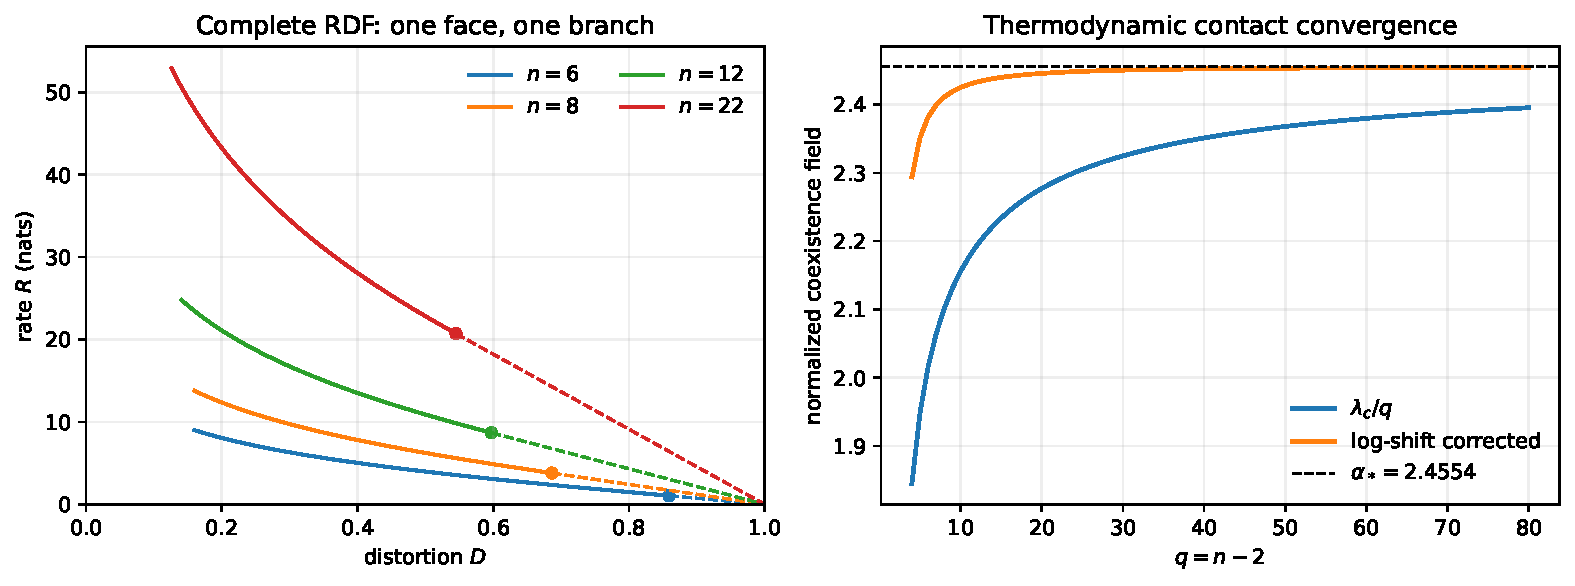
\includegraphics[width=\textwidth]{figures/complete_phase.pdf}
\caption{Left: the exact two-piece RDFs; dots are the unique coexistence
contacts and dashed lines the exact time-sharing faces.  Right: convergence of
the normalized coexistence field, before and after the logarithmic correction
in \cref{eq:lambdashift}.  The plot is diagnostic; every phase and asymptotic
statement is analytic.}
\label{fig:frontier}
\end{figure}

For $n=3$, Hodge duality identifies unit bivectors with $S^2$, and
$L_3=\sinh\kappa/\kappa$ reproduces the known spherical RDF
\cite{DytsoCardone2024}.  For $n=4$,
$\Gr_2^+(\R^4)\simeq S^2\times S^2$; the constrained-gradient argument in
\cref{thm:rdf} is included precisely so that this reducible stabilizer geometry
cannot introduce a hidden posterior-mean component.  In $n=6$, the exceptional
isomorphism $\operatorname{Spin}(6)\simeq SU(4)$ relates the oriented-plane
orbit to $\Gr_{\mathbb C}(2,4)$ and to the exact rank-two companion model
\cite{Eriksson2026RankTwo}.  The present theorem explains why the simple skew
block appears there and extends that mechanism to every real dimension without
relying on the exceptional isomorphism.

The operational object here is a signed Pl\"ucker label.  It can represent an oriented plane or an antisymmetric area coordinate, and squared loss is integrated squared error over an orthonormal basis of linear Pl\"ucker queries.  This is not automatically a quantum-state RDF: a physical ray identifies global sign, and Born probabilities square amplitudes, changing both the sufficient statistic and the loss.  We therefore make no claim about intrinsic randomness, measurement update, click simulation, or a derivation of Born's rule.

\paragraph{Reproducibility.}
The release includes bounded, single-process scripts.  One checks the exact
coefficient signs and parity-binomial reduction; one independently checks the
global-phase identities; one evaluates the exact scalar contacts and their
thermodynamic expansion; and one generates \cref{fig:frontier}.  From the
workspace root:
\begin{verbatim}
powershell -ExecutionPolicy Bypass -File work/twelfth_paper/replay_all.ps1
\end{verbatim}
They are diagnostic replays; no finite screen or floating-point root is used
to prove the all-dimensional theorems.  At the frozen seal, two separate exact
rational replays report 6,783 coefficient-sign checks, 297 boundary-tail
checks, and zero coefficient/binomial-reduction mismatches; the scalar contact
replay extends through $q=120$.  Release seal
\texttt{P12-ARR-UNIFIED-v1} freezes the scripts, JSON diagnostics, and figure
in \path{Eriksson_Paper12_Replay_Artifacts_v1.zip}, whose SHA--256 is
\texttt{\seqsplit{412d36ea2abf9df035d0235064f1b20a6d25c21ac5c50c3f0980005c192bbfd9}}.
The internal file \path{REPLAY_ARTIFACTS.sha256} verifies every replay input
and deterministic output used by the one-command check.

\section{Conclusion}

The parity-binomial coefficient law closes the global phase problem for Haar
oriented-plane compression.  In every dimension six and above the stationary
curve has one fold, the zero and informative phases meet at one positive
contact, and the unique active branch cannot exchange or reenter.  The exact
RDF is therefore one linear coexistence face followed by one covariant branch.
Combined with the continuous cases below dimension six, this is a complete
all-dimensional classification rather than a local cumulant diagnosis.

The unique contact also admits a controlled thermodynamic limit with an
explicit logarithmic finite-size displacement.  At the operational level, the
same curve is the exact minimum worst-source capacity and tensorizes under
arbitrary joint block memory; transitivity supplies a zero-dispersion strong
converse.  The result remains deliberately specific to signed Pl\"ucker
coordinates and squared ambient prediction loss.  Higher exterior degree and
unoriented or quantum reproduction bodies require different spectral
extrema and are not claimed here.

\appendix
\section{Exact algebra in the boundary-tail estimate}\label{app:tailalgebra}

For completeness, the second rational inequality used in
\cref{thm:onechange} is
\[
 \frac75-\frac{P_{r+1}}{P_r}
 =\frac{Q(r-4)}
 {5(r+4)^3(3r+4)(3r+5)(4r+7)^3 H(r)},
\]
where
\[
 H(r)=16r^6+176r^5+753r^4+1591r^3+1943r^2+1353r+440
\]
and
\begin{align*}
Q(u)={}&18432u^{14}+1516032u^{13}+57380608u^{12}
 +1323274880u^{11}+20744953944u^{10}\\
&+233468375862u^9+1940711941655u^8+12066182319572u^7
 +56127825939008u^6\\
&+193034617284784u^5+477660913728601u^4
 +807579069619542u^3\\
&+843129988129352u^2+426935276758816u
 +29229024927872.
\end{align*}
Every coefficient is positive.  This makes the all-$r$ tail step a displayed
rational certificate rather than a finite numerical screen.

\printbibliography
\end{document}
